%! TeX program = lualatex
%---------------------------ALLGEMEINE IMPORTS-------------------------------------
\documentclass[12pt,english,ngerman]{scrartcl}
\input{./protokoll_template/template.latex/input/shared_preamble.tex}

% Kopfzeile
\ihead{WS22\\
	16.12.2022} \chead{\textsc{Stark} Matthias - 12004907 \\
	\textsc{Philipp} Maximilian - 11839611}
\ohead{FLAB 1 \\
	Spektrograph}
% Fußzeile


\begin{document}

\section{Aufgabenstellung\label{sec:Aufgabenstellung}}

\begin{itemize}
	\item Adjustierung des Prismenspektrographen, der Linsen und der Prismen im Spektrographen, um ein Spektrum für alle 
	Lichtquellen abzubilden.
	\item Aufnahme des Spektrums von den Verschiedenen Lichtquellen und der Probe.
	\item Aufnahme der Spektren der gleichen Lichtquellen mit dem Gitterspektrographen.
	\item Erzeugung der Dispersionskurve des Prismenspektrographen.
	\item Bestimmung des Auflösevermögen der beiden Spektrographen.
	\item Bestimmung der Wellenlänge der Jod-Absorbtionsbandkanten.
	\item Bestimmung der Disotiationsenergie des Jodmoleküls.
\end{itemize}

\section{Grundlagen}\label{sec:Grund}


Molekulare Spektroskopie

Wenn elektromagnetische Strahlung mit einem Molekül in Wechselwirkung tritt, kann sie absorbiert, emittiert oder gestreut werden, je nach der Energie der Strahlung und den Energieniveaus des Moleküls. Die Energie der Strahlung wird durch ihre Wellenlänge oder Frequenz bestimmt, und die Energieniveaus des Moleküls werden durch seine elektronische Struktur, seine Vibrations- und Rotationsmoden bestimmt.

Die Absorption oder Emission elektromagnetischer Strahlung durch ein Molekül kann als Änderung der Intensität der Strahlung beim Durchgang durch die Probe beobachtet werden. Diese Änderung kann mit einem Spektrometer gemessen und zur Untersuchung der elektronischen Struktur und Bindung des Moleküls sowie seiner Schwingungs- und Rotationsenergieniveaus verwendet werden.

Prismenspektrograf
Ein Prismenspektrograf ist ein Spektrograf, der ein Prisma verwendet, um die elektromagnetische Strahlung in ihre einzelnen Wellenlängen oder Frequenzen zu zerlegen. Er besteht aus einer Lichtquelle, einem Prisma und einem Detektor und wird verwendet, um das elektromagnetische Spektrum einer Probe grafisch darzustellen.

Die Lichtquelle eines Prismenspektrographen ist in der Regel eine Lampe oder ein Laser, mit dem die Probe beleuchtet wird. Die Probe wird in den Strahlengang gestellt, und ein Teil der elektromagnetischen Strahlung wird von der Probe absorbiert, emittiert oder gestreut.

Das Prisma ist ein transparentes optisches Element, das aus einem brechenden Material wie Glas oder Quarz besteht. Es wird in den Weg der elektromagnetischen Strahlung gestellt und dient dazu, die Strahlung in ihre einzelnen Wellenlängen oder Frequenzen zu zerlegen. Das Prisma funktioniert, indem es die Strahlung je nach Wellenlänge oder Frequenz in unterschiedlichen Winkeln bricht. Dies führt dazu, dass sich die verschiedenen Wellenlängen oder Frequenzen der Strahlung ausbreiten und ein Spektrum bilden.

Der Detektor eines Prismenspektrographen ist in der Regel eine Kamera oder ein Aufzeichnungsgerät, mit dem die Intensität der elektromagnetischen Strahlung über einen Bereich von Wellenlängen oder Frequenzen gemessen wird. Der Detektor erzeugt ein Diagramm der Intensität der Strahlung in Abhängigkeit von der Wellenlänge oder Frequenz, das als Spektrum bezeichnet wird.

Gitterspektrograf
Ein Echelle-Spektrograf ist ein Spektrograf, der ein Beugungsgitter, das so genannte Echelle-Gitter, verwendet, um die elektromagnetische Strahlung in ihre einzelnen Wellenlängen oder Frequenzen zu zerlegen. Er besteht aus einer Lichtquelle, einem Echelle-Gitter, einem Kollimator, einer Kamera oder einem Aufzeichnungsgerät und einer Brennebene.

Bei der Lichtquelle eines Echelle-Spektrographen handelt es sich in der Regel um eine Lampe oder einen Laser, mit dem die Probe beleuchtet wird. Die Probe wird in den Strahlengang gestellt, und ein Teil der elektromagnetischen Strahlung wird von der Probe absorbiert, emittiert oder gestreut.

Das Echelle-Gitter ist ein Beugungsgitter, das aus einem transparenten optischen Element wie Glas oder Quarz besteht und mit einem periodischen Muster aus parallelen Linien versehen ist. Es wird im Strahlengang der elektromagnetischen Strahlung angebracht und dient dazu, die Strahlung in ihre einzelnen Wellenlängen oder Frequenzen zu zerlegen. Das Echelle-Gitter funktioniert, indem es die Strahlung je nach ihrer Wellenlänge oder Frequenz in unterschiedlichen Winkeln beugt. Dies führt dazu, dass sich die verschiedenen Wellenlängen oder Frequenzen der Strahlung ausbreiten und ein Spektrum bilden.

Der Kollimator ist eine Linse oder ein Spiegel, der dazu dient, die elektromagnetische Strahlung zu kollimieren, d. h. zu einem parallelen Strahl zu bündeln. Der Kollimator befindet sich hinter dem Echelle-Gitter und sorgt dafür, dass die Strahlung auf die Kamera oder den Rekorder fokussiert wird.

Mit der Kamera oder dem Rekorder wird die Intensität der elektromagnetischen Strahlung über einen Bereich von Wellenlängen oder Frequenzen gemessen. Es wird ein Diagramm der Strahlungsintensität in Abhängigkeit von der Wellenlänge oder Frequenz erstellt, das als Spektrum bezeichnet wird.

Die Brennebene ist die Ebene, in der das Spektrum gebildet wird, und sie befindet sich in der Regel im Brennpunkt des Kollimators. Die Kamera oder der Rekorder wird in der Fokusebene platziert, um die Intensität der elektromagnetischen Strahlung zu messen.




\section{Versuchsaufbau} \label{sec:aufbau}

\subsection{Prismenspekrograph}

Der Versuchsaufbau ist in folgender \autoref{fig:aufbau_Spektograph} ersichtlich. Dabei wird die Position der Lichtquelle
mit einem leeren Linsenhalter auf der optischen Bank markiert, um später beim Wechsel der Lichtquelle die selbe Position zu
ermöglichen. Bei den Linsen wir dabei versucht, den vorliegenden Lichtstrahl, so gut wie möglich, auf den Eingangsspalt des
Spektrographen zu fokusieren, um eine möglichst hohe Intensität zu gewährleisten. Auch die Position, auf die die Iodzelle
gestellt wird, wird mit einem leeren Linsenhalter markiert.

\begin{figure}[H]
	\begin{center}
		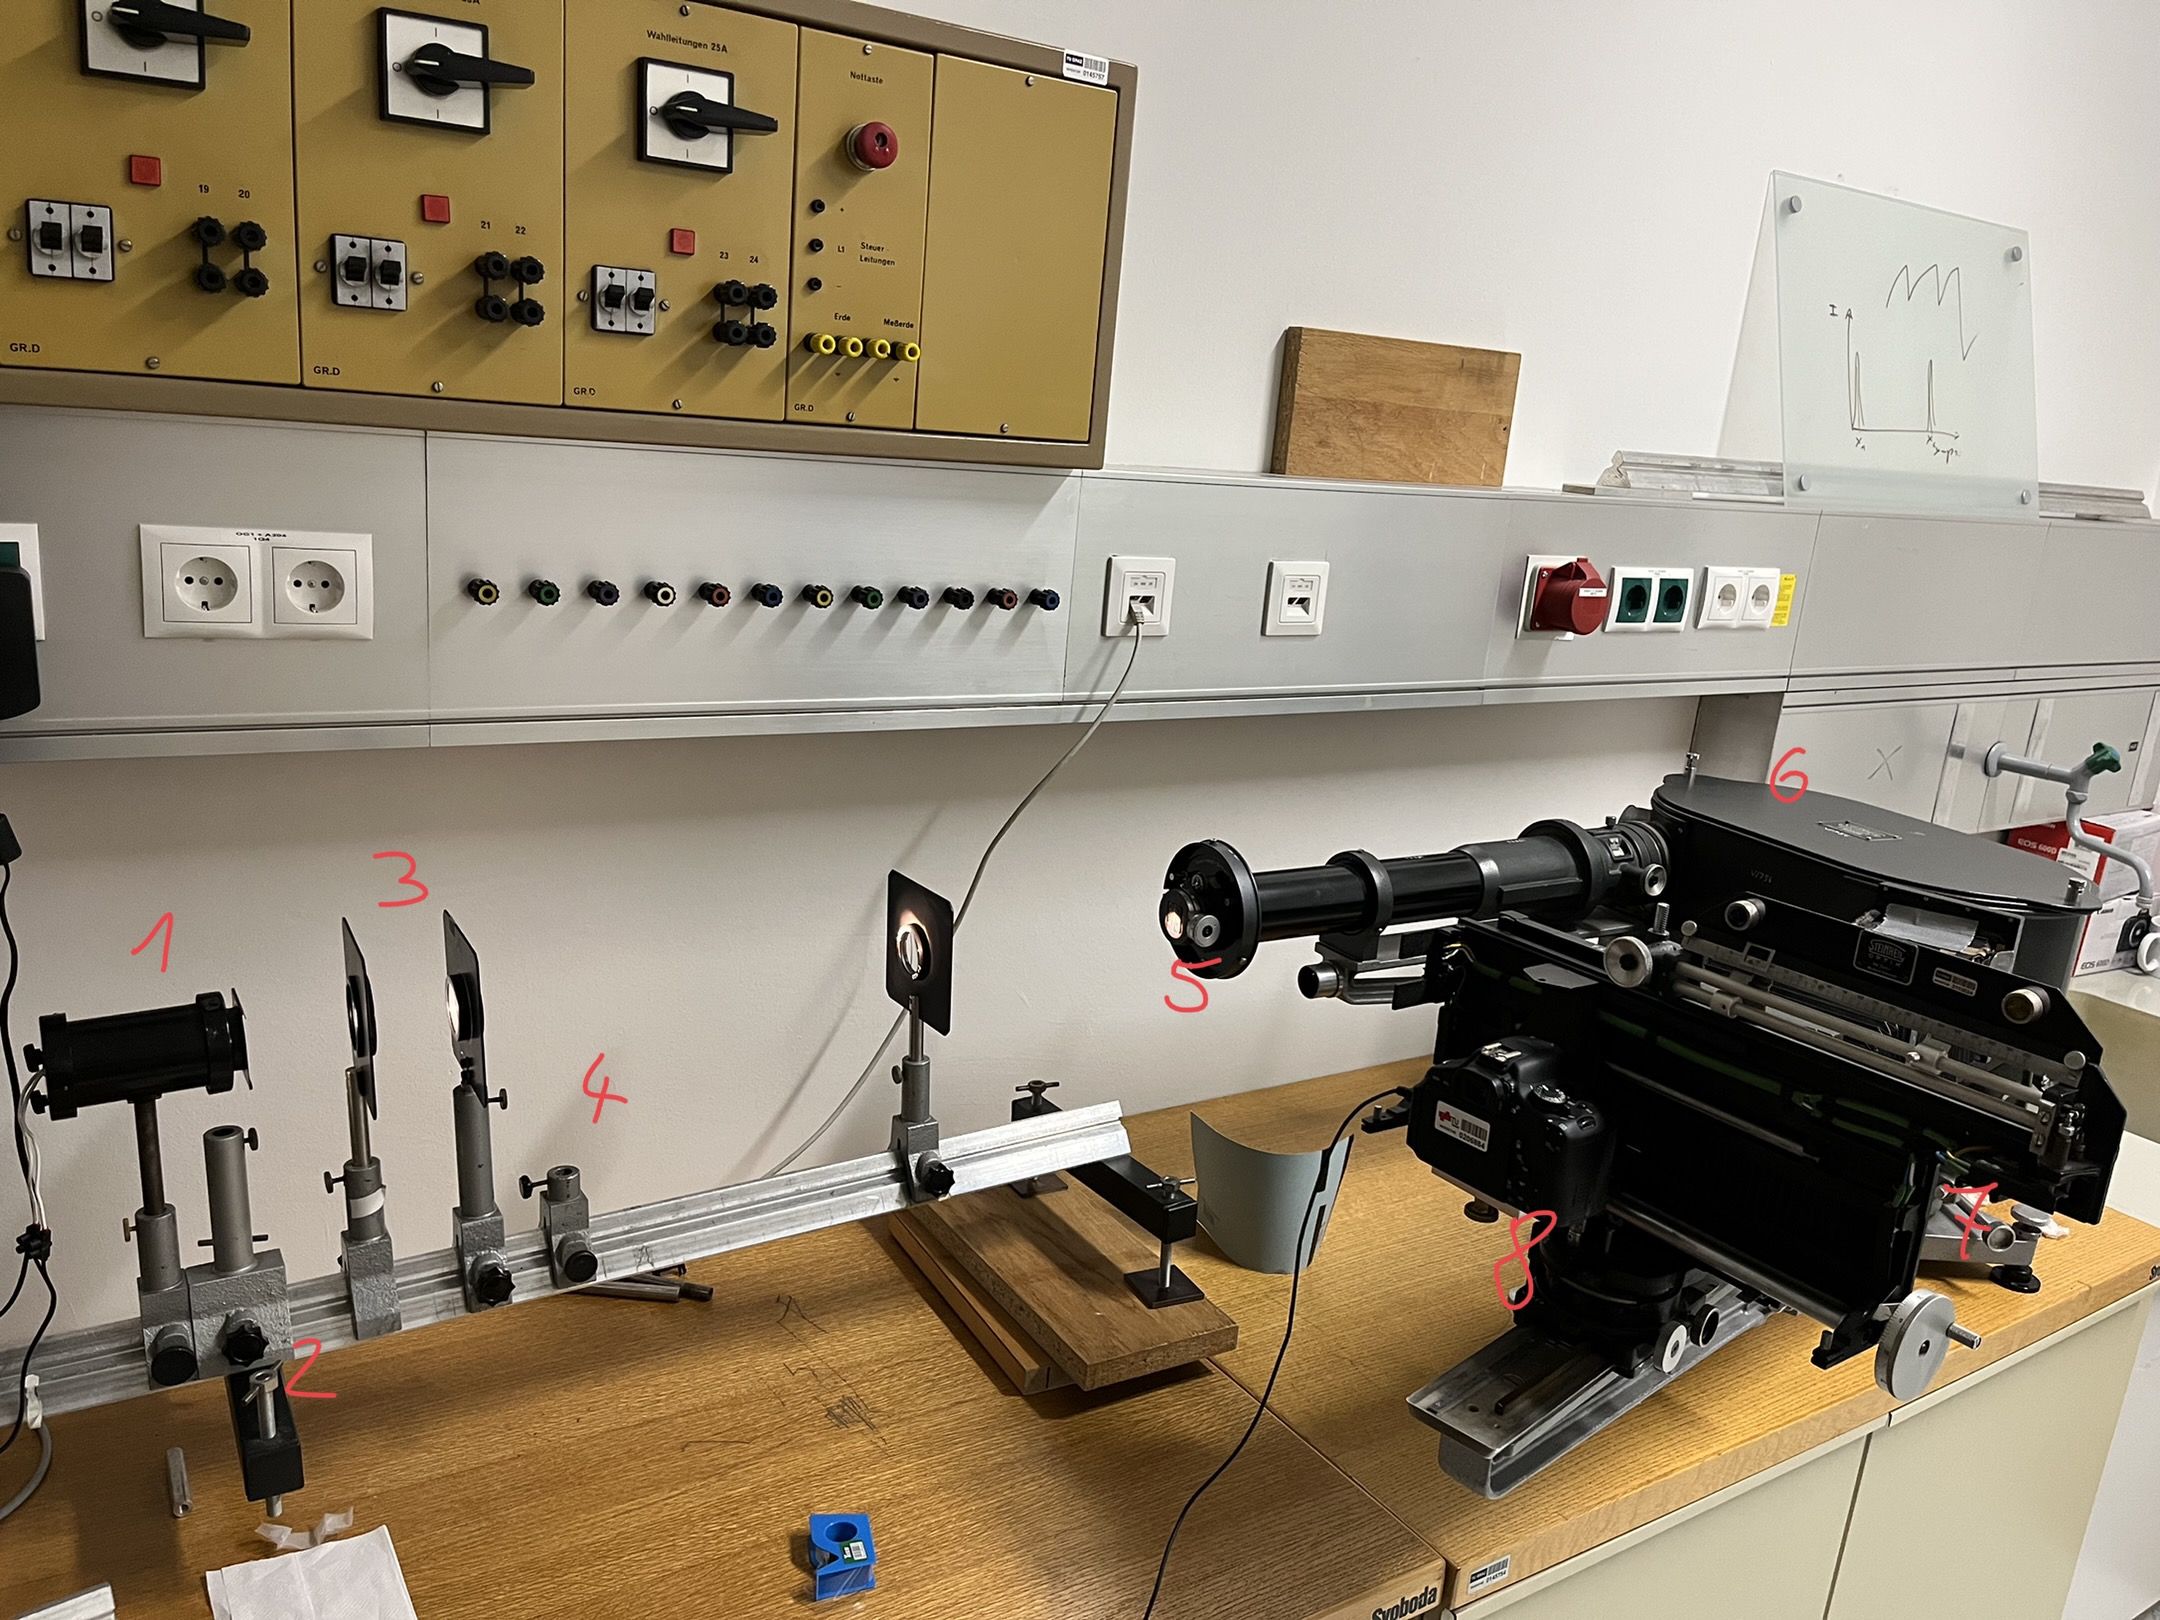
\includegraphics[width =\textwidth]{./figures/Spektograph.png}
	\end{center}
	\caption[Versuchsaufbau des Prismenspektrographen]
	{Versuchsaufbau des Prismenspektrographen \\
	1 \(\dots\) Lichtquelle \\
	2 \(\dots\) Markierung für die Lichtquelle \\
	3 \(\dots\) Verwendete Sammellinsen (Brennweiten: v.l.n.r. 250, 50, 120) \\
	4 \(\dots\) Markierung für die Iodquelle \\
	5 \(\dots\) Eintrittsspalt in den Spektrographen \\
	6 \(\dots\) Prismen in Spektrographen \\
	7 \(\dots\) Halterung für Kamera \\
	8 \(\dots\) Befestigte Kamera
	}\label{fig:aufbau_Spektograph}
\end{figure}

Im inneren des Spektrographen müssen nun die Prismen durch vorsichtiges Verdrehen richtig eingestellt werden, sodass der 
eintreffende Lichtstraht durch die 3 Prismen zur Ausgangsöffnung abgelenkt wird und dort das komplette Spektrum, innerhalb
des Schirms sichtbar ist. Um dies gut beurteilen zu können, wird ein Streifen Klebeband über die entsprehende Öffnung geklebt,
sodass das gebrochene Licht gut sichtbar wird. Die entsprechenden Positionen der Prismen sind in \autoref{fig:prismen} sichtbar.

\begin{figure}[H]
	\begin{center}
		\includegraphics[width =0.5\textwidth]{./figures/Prismen.png}
	\end{center}
	\caption[Anordnung der Prismen im Spektrographen]
	{Anordnung der Prismen im Spektrographen
	}\label{fig:prismen}
\end{figure}

\subsection{Gitterspektograph}

Der Aufbau des Gitterspektrographen ist in \autoref{fig:aufbau_gitter} sichtbar. Dabei wird der Sensor des Gitterspektrographen
mithilfe einer passenden Halterung direkt vor die Lichtquelle gestellt.
\begin{figure}[H]
	\begin{center}
		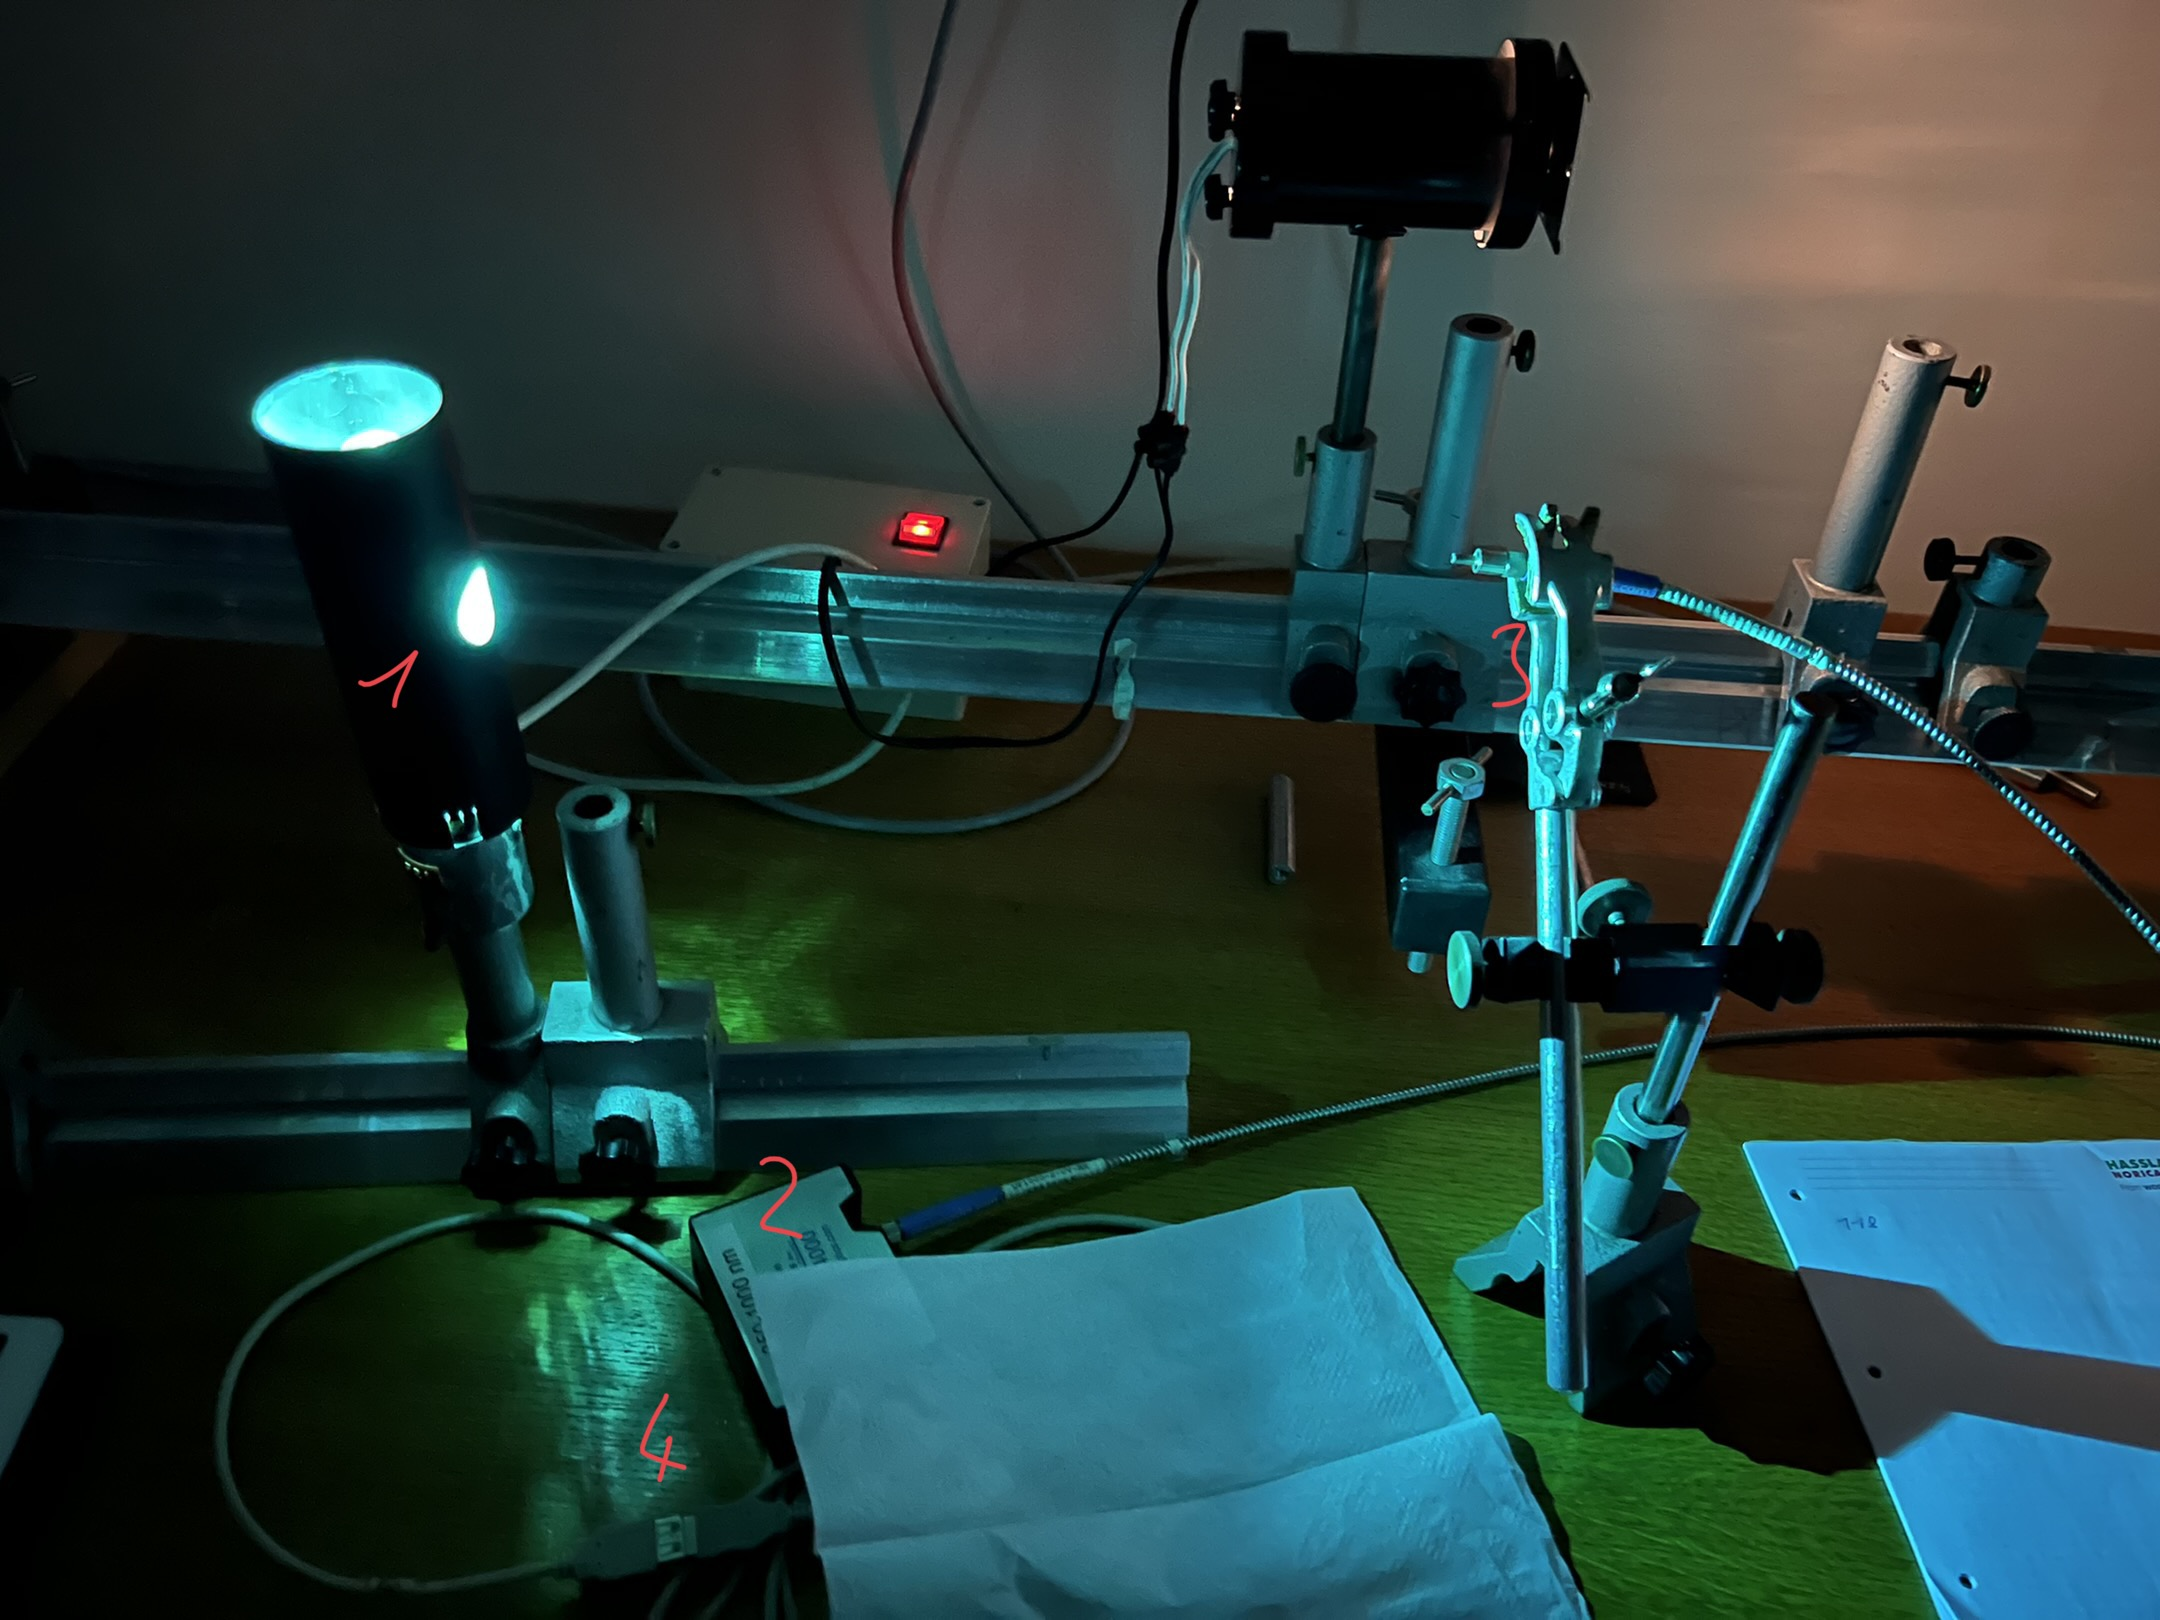
\includegraphics[width =\textwidth]{./figures/Gitterspektograph.png}
	\end{center}
	\caption[Versuchsaufbau des Gitterspektrographen]
	{Versuchsaufbau des Gitterspektrographen \\
	1 \(\dots\) Lichtquelle \\
	2 \(\dots\) Gitterspektograph \\
	3 \(\dots\) Sensor der Spektrographen \\
	4 \(\dots\) Schnittstelle für Computer
	}\label{fig:aufbau_gitter}
\end{figure}


\subsection{Geräte}



\section{Durchführung und Messergebnisse}\label{sec:durchfuhrung}

\subsection{Prismenspekrograph}

Nachdem die Linsen und Prismen wie bereits in \autoref{sec:aufbau} angeführt, aufgebaut wurden,
wird das, von der Kamera erfasste, Spektrum am Computer mit der Software
%todo softwarename
betrachtet. Es ist dafür zu sorgen, dass die einzelnen Linien der Lichtquelle scharf erscheinen und
eine möglichst gute Nutzung der gesamten Breite des zur Verfügung stehenden Schirms vorliegt. Dies wird durch
Verstellen und anschließender Feinjustierung der Neigung und des Abstands der Kamera zum Spektographen 
erreicht.

Weil nicht das gesamte Spektrum mit einem Foto aufgezeichnet werden kann wird zunächst bestimmt, wie groß der 
erfasste Bereich ist. Dazu wird zunächst die Kamera mithilfe der entsprechenden Kurbel so lange bewegt, bis der
rote Peak gerade am rechten Rand des Bildschirms verschwindet. Nun wird die Kamera, unter Bestimmung der entsprechenden 
Distanz, solange weiterbewegt, bis sich diese rote Linie am linken Rand des Bildschirms befindet. Dadurch wird die 
Distanz des aufgezeichneten Spektrums bestimmt. Nun wird auf diese Art das gesamte Spektrum aufgezeichnet, welches
schließlich Bild für Bild zusammengesetzt werden kann. Dabei ist zu beachten, dass das Spektrum immer von beiden 
Lichtquellen und der Iodprobe festgehalten wird, bevor die Kameraposition verschoben wird. Weil bei den verschiedenen 
Farbeindrücken unterschiedliche Helligkeiten vorliegen, muss auch immer der Kontrast neu eingestellt werden.
Ein Bild eines Teils des Spektrums ist symbolisch in folgender \autoref{fig:comp} sichtbar.


%todo foto vom comp programm \label{fig:comp}



\subsection{Gitterspektograph}


\section{Auswertung}\label{sec:auswertung}


\subsection{Dispersionskurve des Prismenspektrographen}


\subsection{Auflösevermögen}


\subsection{Wellenlänge der Jod-Absorbtionsbandkanten}


\subsection{Disotiationsenergie des Jodmoleküls}


\section{Diskussion}\label{sec:disk}


\subsection{Dispersionskurve des Prismenspektrographen}


\subsection{Auflösevermögen}


\subsection{Wellenlänge der Jod-Absorbtionsbandkanten}


\subsection{Disotiationsenergie des Jodmoleküls}


\section{Zusammenfassung}\label{sec:zs}


\subsection{Dispersionskurve des Prismenspektrographen}


\subsection{Auflösevermögen}


\subsection{Wellenlänge der Jod-Absorbtionsbandkanten}


\subsection{Disotiationsenergie des Jodmoleküls}










\end{document}